\documentclass{article}
\usepackage{graphicx} % Required for inserting images
\usepackage{amsmath}
\usepackage[russian]{babel}
\usepackage{float}


\renewcommand{\thesection}{\arabic{section}}

\title{Методы оптимизации, Лабораторная работа №4}
\author{Кирилл Кадомцев}
\date{Май 2025}
\setlength{\parindent}{0pt}
\begin{document}
\maketitle
\tableofcontents

\section{Описание}
Был реализован метод симуляции отжига с возможностью выбора различных гиперпараметров


\newpage

\section{Тестирование}
В первую очередь, для тестирования были выбраны зашумлённые функции, на которых методы из предыдущих лабораторных банально не смогли вычислить результат, в то время как метод симуляции отжига должен быть устойчив:

\textbf{Периодическая зашумлённая функция:} \\
\[f(x) = \sin(x) + 0.5 \cdot \sin(3x) + \text{Noise}(x)\text{, где Noise}(x) = 0.1 \cdot \sin(20x) + 0.05 \cdot \mathcal{N}(0, 1)\]
\begin{figure}[H]
    \centering
    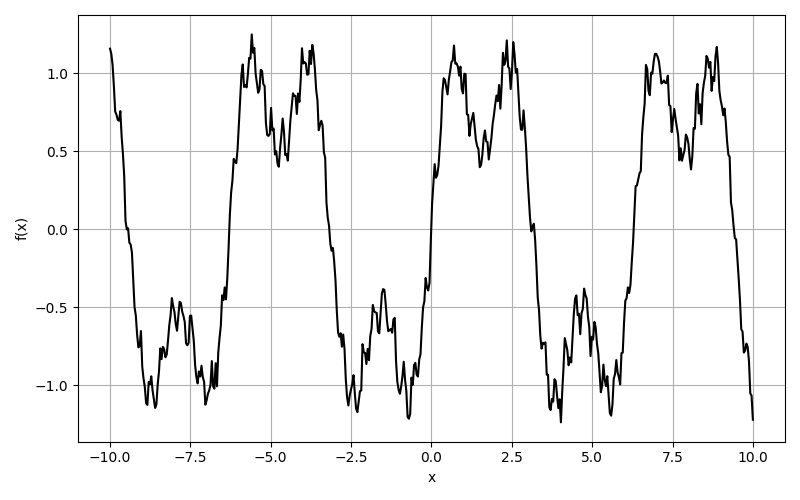
\includegraphics[width=0.5\linewidth]{noisy_periodic.png}
\end{figure} \\
\textbf{Непериодическая зашумлённая функция:} \\
\[f(x) = 0.02x^2 - 0.5x + \underbrace{0.3 \cdot e^{-0.5(x - 2)^2} - 0.4 \cdot e^{-0.3(x + 3)^2}}_{\text{локальные "бугры"}} + \underbrace{0.1 \cdot \mathcal{N}(0,1)}_{\text{шум}}\]
\begin{figure}[H]
    \centering
    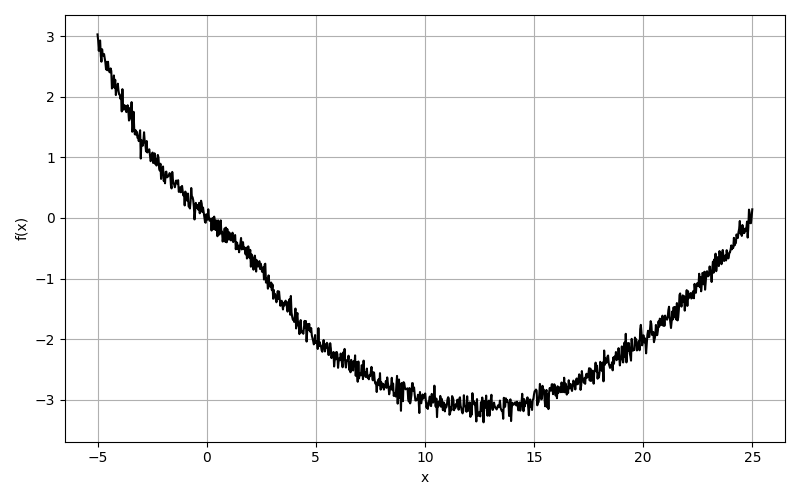
\includegraphics[width=0.5\linewidth]{noisy_nonperiodic.png}
\end{figure}

Также, некоторые другие функции, использовавшиеся для тестирования:

\begin{itemize}
    \item Параболоид: $f(x, y) = x^2 + y^2$
    \item Функция Розенброка: $f(x, y) = (1 - x)^2 + 100 \cdot (y - x^2)^2$
    \item Квадратичная форма (min3m2): $f(x, y) = (x - 3)^2 + (y + 2)^2$
    \item Квадратичная форма (min2m1): $f(x, y) = x + y$
    \item Функция Химмельблау: $f(x, y) = (x^2 + y - 11)^2 + (x + y^2 - 7)^2$
\end{itemize}


\section{Результаты тестирования}
Важно отметить, что тестирования производилось с ограничением в 100000 итераций

\subsection{В зависимости от параметра $\alpha$ (коэффициент остывания)}
\begin{table}[H]
\centering
\begin{tabular}{|c|c|c|}
\hline
\textbf{Alpha} & \textbf{Best $x$} & \textbf{Function Value} \\
\hline
0.5 & [-2075.733258386746] & -1.143854 \\
0.9 & [-580.2988103253542] & -1.073550 \\
0.99 & [1255.971884522375] & -1.092126 \\
\hline
\end{tabular}
\caption{noisy\_periodic (start t=1000, final t=0.001)}
\end{table}
\begin{table}[H]
\centering
\begin{tabular}{|c|c|c|}
\hline
\textbf{Alpha} & \textbf{Best $x$} & \textbf{Function Value} \\
\hline
0.5 & [12.76986017115421] & -3.027205295394961 \\
0.9 & [13.000829261723327] & -3.1884971716494124 \\
0.99 & [11.54719088183137] & -2.931912130302153 \\
\hline
\end{tabular}
\caption{noisy\_nonperiodic (start t=1000, final t=0.001)}
\end{table}
В итоге лучшим значением оказалось среднее. В первом случае, скорость остывания была слишком быстрой и функция "застряла", во втором - слишком медленной и упёрлась в количество итераций.

\subsection{В зависимости от \textit{start\_t}}
\begin{table}[H]
\centering
\begin{tabular}{|c|c|c|}
\hline
\textbf{Start $t$} & \textbf{Best $x$} & \textbf{Function Value} \\
\hline
100 & [24.44007420608933] & -1.175309 \\
1000 & [-580.2988103253542] & -1.073550 \\
\hline
\end{tabular}
\caption{noisy\_periodic ($\alpha=0.9$, $final\_t=0.001$)}
\end{table}
\begin{table}[H]
\centering
\begin{tabular}{|c|c|c|}
\hline
\textbf{Start $t$} & \textbf{Best $x$} & \textbf{Function Value} \\
\hline
100 & [12.774633155205372] & -3.177636 \\
1000 & [13.000829261723327] & -3.188497 \\
\hline
\end{tabular}
\caption{noisy\_nonperiodic ($\alpha=0.9$, $final\_t=0.001$)}
\end{table}


\subsection{В зависимости от \textit{final\_t}}
\begin{table}[H]
\centering
\begin{tabular}{|c|c|c|}
\hline
\textbf{Final $t$} & \textbf{Best $x$} & \textbf{Function Value} \\
\hline
1e-3 & [-580.2988103253542] & -1.073550 \\
1e-5 & [-220.62114482011734] & -1.043032 \\
\hline
\end{tabular}
\caption{noisy\_periodic ($\alpha=0.9$, $start\_t=1000$)}
\end{table}
\begin{table}[H]
\centering
\begin{tabular}{|c|c|c|}
\hline
\textbf{Final $t$} & \textbf{Best $x$} & \textbf{Function Value} \\
\hline
1e-3 & [13.000829261723327] & -3.188497 \\
1e-5 & [12.488401777145537] & -3.113249 \\
\hline
\end{tabular}
\caption{noisy\_nonperiodic ($\alpha=0.9$, $start\_t=1000$)}
\end{table}

Результат ухудшился - алгоритм застревал в локальных минимумах при слишком медленном замораживании



\section{Метаоптимизация}
Метод отжига был применён для оптимизации размера батча для предыдущей лабораторной. При ограничении итераций для линейной регрессии в 100 закономерно выдавался результат 1, данный тест ничего особо не показывает. В то время как при 1000 оптимальным оказался размер батча в 35.
\end{document}